\documentclass[aspectratio=169]{beamer}
\usetheme{Madrid}
\usepackage[utf8]{inputenc}
\usepackage[T1]{fontenc}
\usepackage{tikz}
\usepackage{amssymb}
\usepackage{graphicx}
\setbeamertemplate{navigation symbols}{}
\setbeamercolor{title}{fg=white,bg=green!55!teal}
\setbeamercolor{frametitle}{fg=white,bg=green!55!teal}
\setbeamercolor{block title}{bg=green!55!teal!20,fg=black}
\setbeamercolor{block body}{bg=green!55!teal!8,fg=black}
\setbeamercolor{item}{fg=green!55!teal}
\setbeamercolor{itemize item}{fg=green!55!teal}
\setbeamertemplate{itemize item}[triangle]

\title{M3 — Functions}
\subtitle{def, parameters, return — refactor copy-paste into reusable powers}
\author{ByteForge --- Grade 8 --- App Builder}
\date{}

\begin{document}

\begin{frame}
    \titlepage
\end{frame}

\begin{frame}{Today's Plan}
    \begin{itemize}
        \item Functions with Parameters
        \item A Loop That Calls a Function
        \item return — Handing Back a Value
        \item A Function With a Loop Inside
        \item Returning More Than One Value
        \item[$\bigstar$] BOSS --- M3 Capstone
    \end{itemize}
\end{frame}

\begin{frame}{def name(params): — the real syntax for "My Blocks"}
    \large
    \begin{itemize}
        \item \texttt{def draw\_smiley(x, y, r, ...):} defines a reusable function, exactly like Grade 7's custom blocks
        \item Just typed instead of dragged.
    \end{itemize}

    \begin{center}
    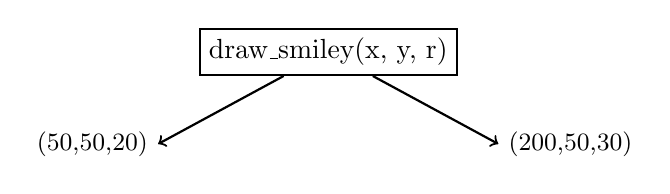
\begin{tikzpicture}[scale=0.9]

        \node[draw, thick, minimum width=3.2cm] (f) at (0,0) {draw\_smiley(x, y, r)};
        \draw[->, thick] (f) -- (-2.4,-1.3) node[left]{\small (50,50,20)};
        \draw[->, thick] (f) -- (2.4,-1.3) node[right]{\small (200,50,30)};
    \end{tikzpicture}
    \end{center}
\end{frame}


\begin{frame}{A loop that calls a function repeatedly}
    \large
    \begin{itemize}
        \item Calling \texttt{colored\_tile(...)} inside a \texttt{for} loop, with different x/y each time, builds a whole grid from ONE function definition.
    \end{itemize}
\end{frame}


\begin{frame}{return — a function that hands back a value}
    \large
    \begin{itemize}
        \item \texttt{average(a, b, c)} computes a VALUE and hands it back with \texttt{return}, to be used however the caller wants
        \item \texttt{r = average(20, 60, 100)} captures it.
    \end{itemize}
\end{frame}


\begin{frame}{A function with a loop INSIDE it}
    \large
    \begin{itemize}
        \item \texttt{is\_prime(n)} has a real \texttt{for} loop inside its own definition
        \item \texttt{return} exits IMMEDIATELY, even mid-loop, the moment the answer is known.
    \end{itemize}
\end{frame}

\begin{frame}{Real-World Examples}
    \large
    \begin{itemize}
        \item Minecraft's real \texttt{/function} command lets you name and reuse a whole set of commands, called from anywhere
        \item The exact same idea, just in the game's own scripting system rather than Python.
    \end{itemize}
\end{frame}


\begin{frame}{Image}
    \begin{center}
    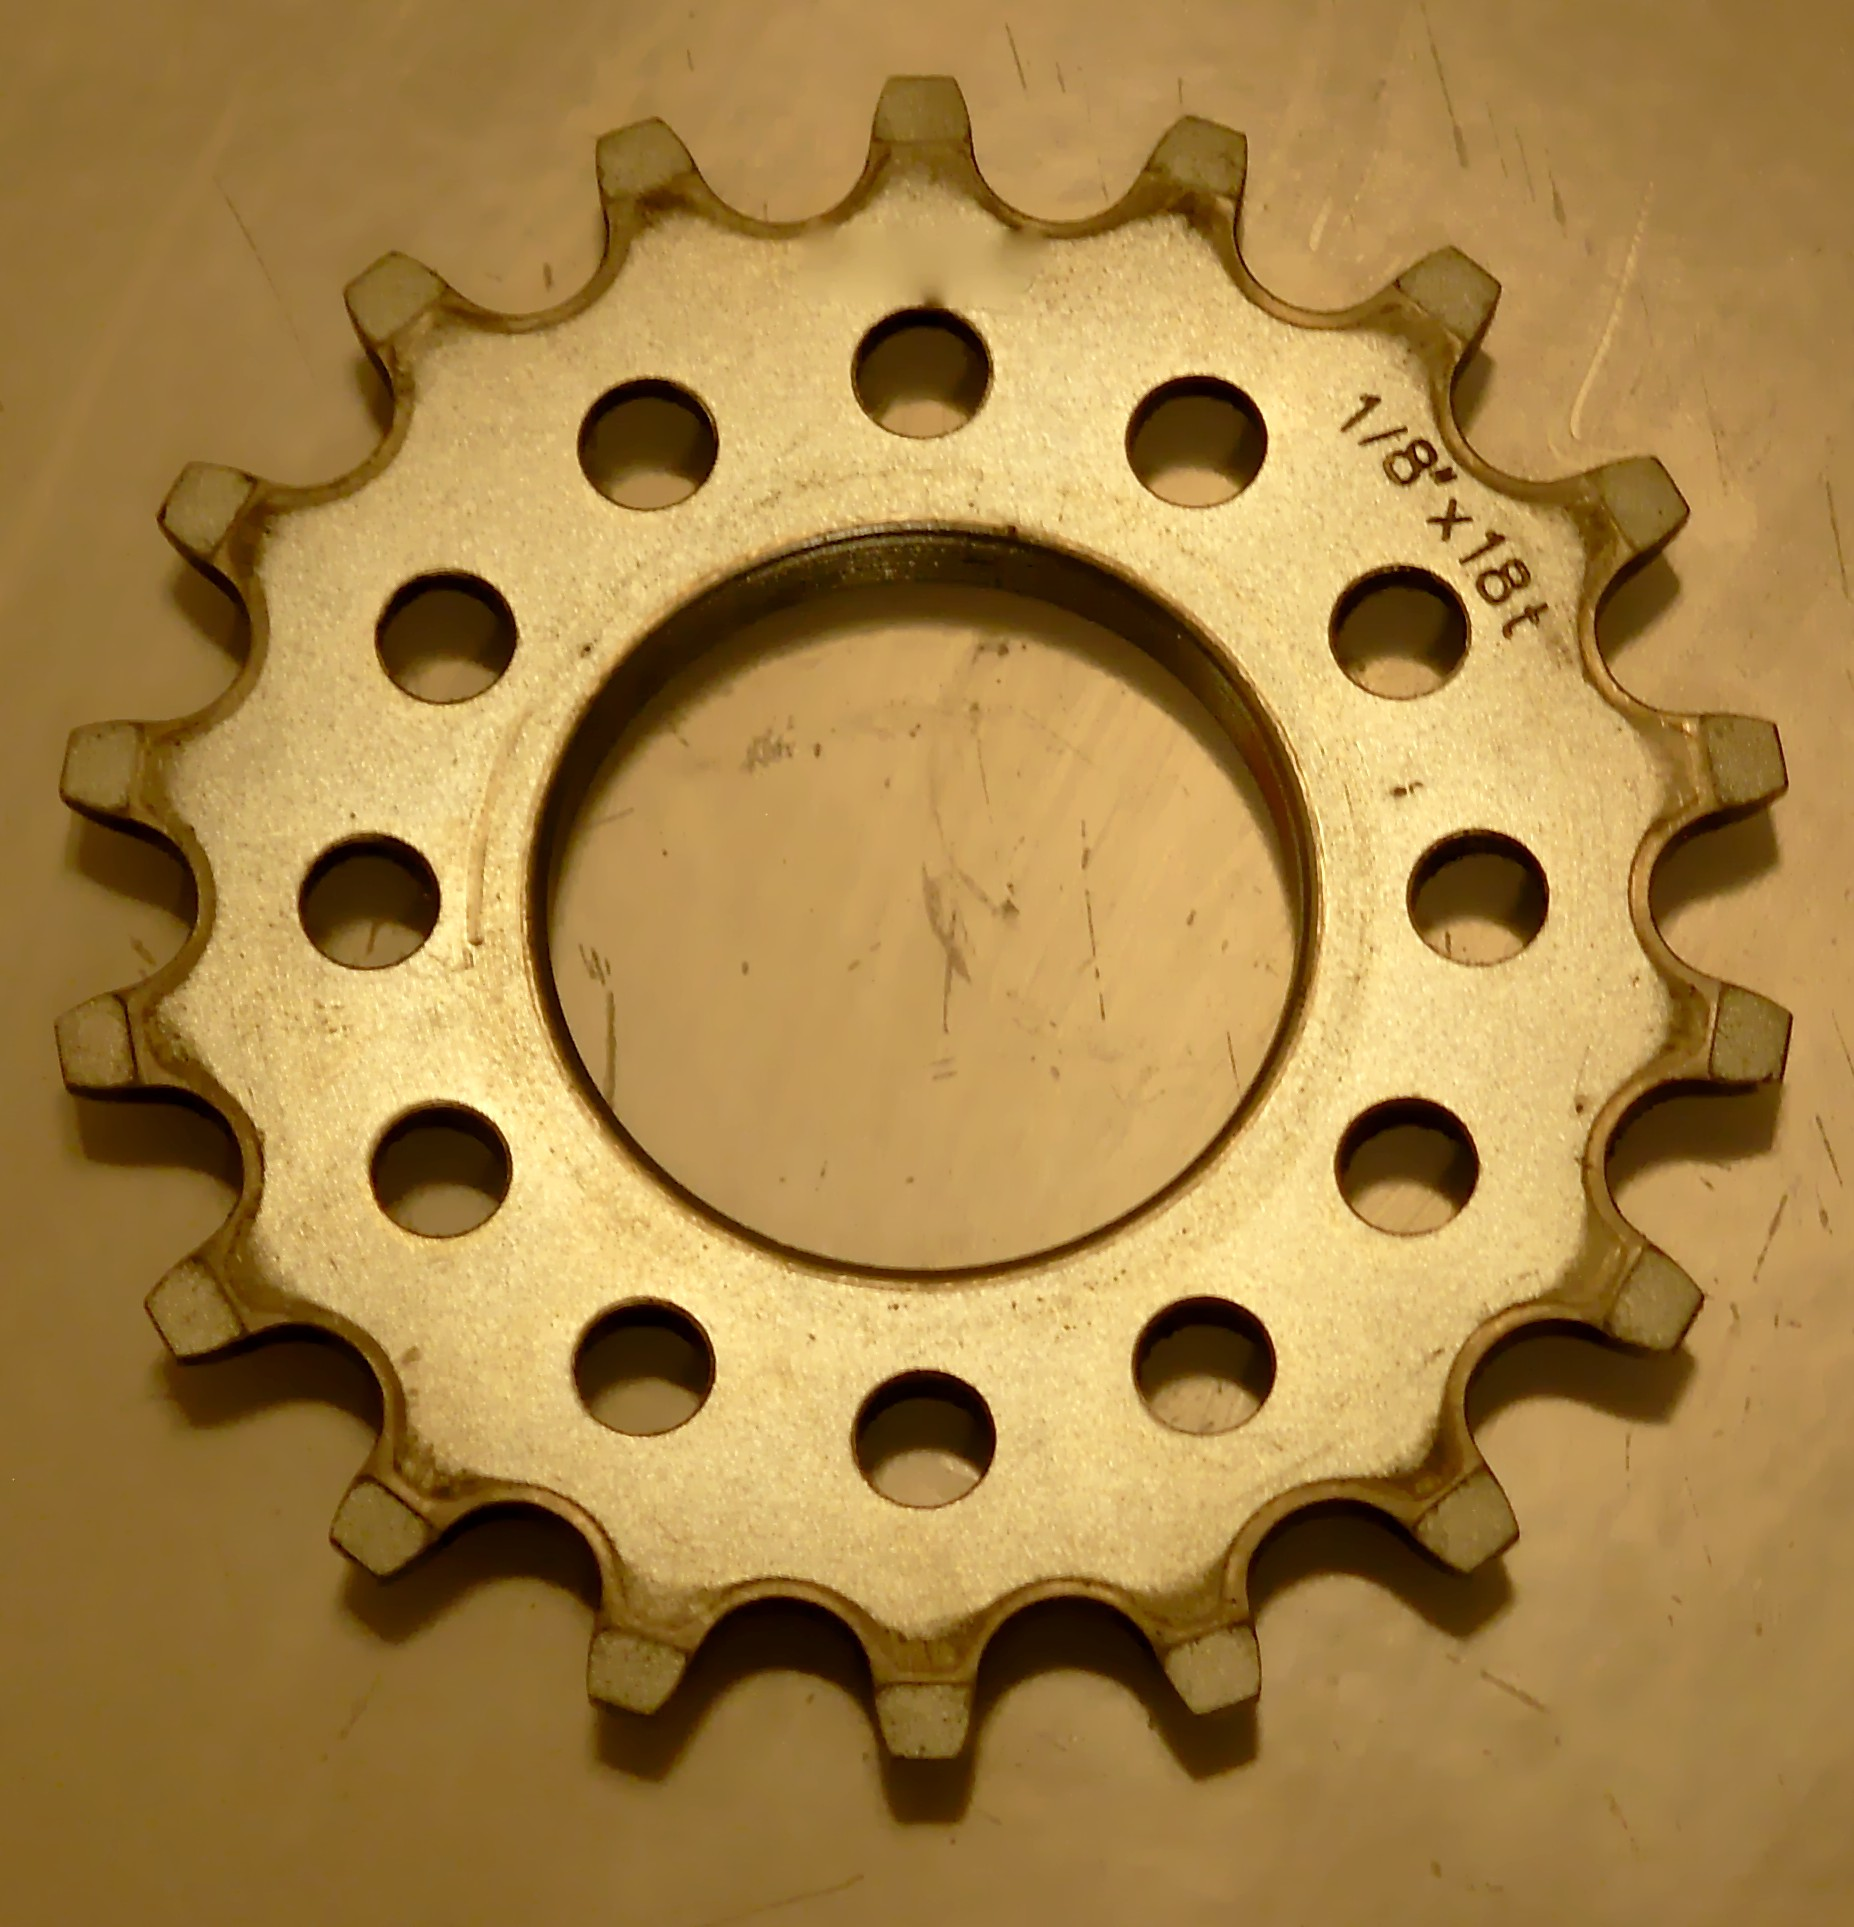
\includegraphics[width=0.5\textwidth]{images/gear.jpg}

    \large Same idea as Web Story 2's image --- one defined job, called repeatedly with different inputs.

    \small Fixed gear cog — John Reaves, public domain, via Wikimedia Commons
    \end{center}
\end{frame}

\begin{frame}{Let Them Discover}
    \Large
    Think of a calculation you might reuse often (a tip calculator, a grade average). Write just its NAME and what it needs as input (parameters) — you've just designed a function's signature before writing a single line inside it.
\end{frame}

\begin{frame}{Your Turn}
    \Large
    Open the student map, find \textbf{M3 — Functions}, and work through it
    hands-on --- everything you just saw, they now do themselves.
\end{frame}

\end{document}
